%!TEX root = ../Thesis.tex
\chapter{Introduction}
\noindent According to the International Energy Agency \cite{iea}, providing heating for homes and industrial purposes accounts for around 50\% of the total energy consumption in the world. Renewable heat consumption in the form of bioenergy contribution is expected to grow which will be a better solution for the climate. In relation to the individual consumer, it makes sense to become aware of one's heat consumption. Many consumers can save money on their heat consumption by making small adjustments such as replacing radiators with more efficient cooling, replacement of leaky windows, improve insulation of the house etc. Which factors that can influence the heat consumption are not known to most consumers and it can be challenging to know how to minimize the consumption. \\

\noindent Heat consumption can be described using mathematical models, namely statistical models, and this can lead to an optimization of the consumption. 
By examining the influence of different physical phenomena on heat consumption, including the temperature, the wind, the sun etc. the properties of a house can be interpreted and visualised for consumers.

\section{Introduction to WATTS App}
\begin{wrapfigure}{r}{0.5\textwidth}
    \vspace{-20pt}
      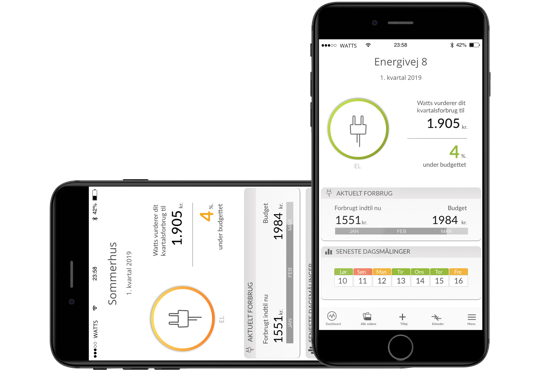
\includegraphics[width=0.48\textwidth]{../../../figures/Watts.png}
    \vspace{-10pt}
  \end{wrapfigure}
The app WATTS is designed and created by the danish energy and optical fibre broadband concern, SEAS-NVE. The app provides several features to the consumer, including an overview of the energy consumption, by showing the actual consumption and predicting the expected future consumption. 
In addition, the app keeps track of the consumers budget and gives the user the opportunity to compare their consumption with similar consumers. The energy consumption in relation to the expected consumption is visualised with the colours green, yellow and red. The colours are used to indicate whether the consumption is expected to be lower than expected, to exceed the budget by 0-30\%, or to exceed the budget by more than 30\%.
\noindent The app is under expansion such that users are offered the same applications for their heat consumption. This paper proposes different features for this expansion, for example it is possible to illustrate the wind dependency on the heat consumption.

\section{Motivation}
The aim of this report is to investigate the tap water consumption and thereby provide possible extensions to WATTS. By illustrating these features in the app, customers can become aware of their heat consumption and at the same time get a sense of what physical phenomena affect their house. 
\noindent Last but not least, a big part of the motivation is driven by the collaboration with a company that focuses on making the energy sector more sustainable. This project contributes to that goal by trying to help the consumer reduce their own consumption. \\

\noindent Our approach is to develope statistical models in order to analyse which factors influence the heat consumption. First we will explore the data as daily values and use linear regression models for fitting and predicting with the main focus on the estimates for various significant parameters. Subsequently, we will do a more indepth analysis of data by examining hourly values. The aim is to determine whether the estimates of the different parameters can be improved. 
